% Created 2024-02-03 Sat 10:41
% Intended LaTeX compiler: pdflatex
\documentclass[11pt]{article}
\usepackage[utf8]{inputenc}
\usepackage[T1]{fontenc}
\usepackage{graphicx}
\usepackage{longtable}
\usepackage{wrapfig}
\usepackage{rotating}
\usepackage[normalem]{ulem}
\usepackage{amsmath}
\usepackage{amssymb}
\usepackage{capt-of}
\usepackage{hyperref}
\usepackage{placeins}
\usepackage{gensymb}
\author{Christian Johnson\and Dan Nusraty\and Dylan Mcgill\and\newline Mailroom 2.0}
\date{\today}
\title{Mail Database Project}
\hypersetup{
 pdfauthor={Christian Johnson\and Dan Nusraty\and Dylan Mcgill\and\newline Mailroom 2.0},
 pdftitle={Mail Database Project},
 pdfkeywords={},
 pdfsubject={},
 pdfcreator={Emacs 28.2.50 (Org mode 9.7-pre)}, 
 pdflang={English}}
\begin{document}

\maketitle
\section{Contents}
\label{sec:org76da9f8}
\subsection{Functional Requirements}
\label{sec:orge35fa85}
\subsection{Non Functional Requirements}
\label{sec:org7d1b51f}
\subsection{Use Case Diagram}
\label{sec:org989843c}
\subsection{Individual Use Cases}
\label{sec:org0a0813c}
\subsubsection{Dan}
\label{sec:org0785e5a}
\subsubsection{Christian}
\label{sec:orgb688143}
\subsubsection{Dylan}
\label{sec:org2bb8642}
\subsection{Meeting Summaries}
\label{sec:org930a0f0}
\clearpage
\section*{Functional Requirements}
\label{sec:org8fb7166}
\begin{itemize}
\item Accept data entry
\item Record tracking number and addressed box number for incoming packages
\item Add entered information into sql database
\item Associate incoming packages with Cadet information based on addressed box number
\item Notify Cadet upon package arrival
\item Record package status (Picked up or not)
\item Search database for packages
\item Display all packages matching search terms
\item Easily update package status
\item Developers will write code in an organized fashion, such that the system is easy to expand later.
\end{itemize}
\section*{Non Functional Requirements}
\label{sec:org2351dff}
\begin{itemize}
\item Will not misassociate packages
\item Will allow package entry, given necessary data, within 5 seconds
\item Will be easily navigable, with all system functions available within 5 clicks
\item Will allow package retrieval, given sufficient search information, within 10 seconds
\item Will never fail to retrieve Cadet information, given sufficient correct search information
\item Will never allow a package entry without associated Cadet information and association
\end{itemize}
\section*{Use Case Diagram}
\label{sec:org5df28f7}

\begin{figure}[htbp]
\centering
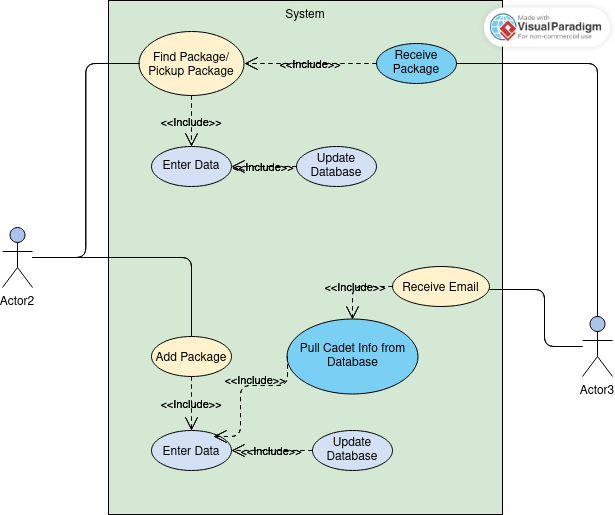
\includegraphics[width=.9\linewidth]{/home/csj7701/Projects/Mail-Database-Project/Class-Documents/Requirements_UseCaseDiagram.png}
\bicaption{.                        Actor 2: Employee, Actor 3: Cadet }
\end{figure}
\newpage
\section*{Individual Use Cases}
\label{sec:orgabb011d}
test
\subsection*{Dan}
\label{sec:org5251007}
Receive Package
\subsection*{Christian}
\label{sec:org0ba6888}
test
\subsection*{Dylan}
\label{sec:org7cc8100}
test
\section*{Meeting Summaries}
\label{sec:orged2ca6f}
\subsection*{Meeting 1 - 30JAN2024}
\label{sec:orgfd3e0cd}
\begin{itemize}
\item Decided on division of labor
\item Agreed on general project scope
\item Began formulating Functional Requirements
\end{itemize}
\subsection*{Meeting 2 - 01FEB2024}
\label{sec:org6167109}
\begin{itemize}
\item Created Use-Case Diagram
\item Finished Functional Requirements
\item Started Non Functional
\item Started individual Use Cases
\end{itemize}
\subsection*{Meeting 3 - 02FEB2024}
\label{sec:orga09bea0}
\begin{itemize}
\item Polished Use-Case Diagram
\item Completed Requirements
\item Finished Individual Components
\end{itemize}
\end{document}